% --------------------------------------------------------------
% This is all preamble stuff that you don't have to worry about.
% Head down to where it says "Start here"
% --------------------------------------------------------------
 
\documentclass[12pt]{article}

\usepackage{courier}
\usepackage{color}
\usepackage{listings}
\usepackage[square,numbers]{natbib}
\usepackage{tabls}
\usepackage{graphicx}
\usepackage{subcaption}
\usepackage{pdfpages}
\usepackage{mathtools}
\usepackage{enumitem}
\usepackage{hyperref}
\usepackage{multirow}
\definecolor{dkgreen}{rgb}{0,0.6,0}
\definecolor{gray}{rgb}{0.5,0.5,0.5}




\lstset{language=Matlab,
   keywords={break,case,catch,continue,else,elseif,end,for,function,
      global,if,otherwise,persistent,return,switch,try,while},
   basicstyle=\ttfamily,
   keywordstyle=\color{blue},
   commentstyle=\color{red},
   stringstyle=\color{dkgreen},
   numbers=left,
   numberstyle=\tiny\color{gray},
   stepnumber=1,
   numbersep=10pt,
   backgroundcolor=\color{white},
   tabsize=4,
   showspaces=false,
   showstringspaces=false}
 
\usepackage[margin=1in]{geometry} 
\usepackage{amsmath,amsthm,amssymb}
\usepackage{verbatim}
\usepackage{algpseudocode}
\usepackage{algorithm}
\usepackage{setspace}

\newcommand{\lline}{\noindent\makebox[\linewidth]{\rule{\textwidth}{0.4pt}}}
\newcommand{\N}{\mathbb{N}}
\newcommand{\Z}{\mathbb{Z}}
\newcommand{\deriv}[2]{\frac{\mathrm{d} #1}{\mathrm{d} #2}}
\newcommand{\pderiv}[2]{\frac{\partial #1}{\partial #2}}
\newcommand{\bx}{\mathbf{X}}
\newcommand{\ba}{\mathbf{A}}
\renewcommand{\d}{\mathrm{d}}
\newcommand{\upl}{u_{\text{plane}}}
\newcommand{\upt}{u_{\text{point}}}
\newcommand{\D}{\Delta}
\renewcommand{\SS}{\State}
\graphicspath{{figures/},{drawing/}}
 
\newenvironment{theorem}[2][Theorem]{\begin{trivlist}
\item[\hskip \labelsep {\bfseries #1}\hskip \labelsep {\bfseries #2.}]}{\end{trivlist}}
\newenvironment{lemma}[2][Lemma]{\begin{trivlist}
\item[\hskip \labelsep {\bfseries #1}\hskip \labelsep {\bfseries #2.}]}{\end{trivlist}}
\newenvironment{exercise}[2][Exercise]{\begin{trivlist}
\item[\hskip \labelsep {\bfseries #1}\hskip \labelsep {\bfseries #2.}]}{\end{trivlist}}
\newenvironment{problem}[2][Problem]{\begin{trivlist}
\item[\hskip \labelsep {\bfseries #1}\hskip \labelsep {\bfseries #2:}]\hspace{0.3in}\newline\newline}{\end{trivlist}}
\newenvironment{question}[2][Question]{\begin{trivlist}
\item[\hskip \labelsep {\bfseries #1}\hskip \labelsep {\bfseries #2.}]}{\end{trivlist}}
\newenvironment{corollary}[2][Corollary]{\begin{trivlist}
\item[\hskip \labelsep {\bfseries #1}\hskip \labelsep {\bfseries #2.} ]}{\end{trivlist}}
\newenvironment{problem*}[1][Problem]{\begin{trivlist}
\item[\hskip \labelsep {\bfseries #1} {\hspace{-0.2em}\bfseries:}]}{\end{trivlist}}
\newenvironment{solution}[1][Solution]{\begin{trivlist}
\item[\hskip \labelsep {\bfseries #1} {\hspace{-0.2em}\bfseries:}]\hspace{0.3in}\newline}{\end{trivlist}}
 
\begin{document}
 
% --------------------------------------------------------------
%                         Start here
% --------------------------------------------------------------
 
\title{Project Report: A Comparison of Parallel Domain Copy and Decomposition for a
1D Monte Carlo Transport Code}%replace X with the appropriate number
\author{Simon Bolding\\ %replace with your name
CSCE 626} %if necessary, replace with your course title
 
\maketitle

\clearpage

%\includepdf[pages={1}]{p1p3.pdf}

\section*{References}

\begin{enumerate}
	\item People in class - Daniel Holladay
	\item wikipedia.org/wiki/Prefix\_sum,computing.llnl.gov, mpitutorial.com
    \item EOS website: sc.tamu.edu/systems/eos
\end{enumerate}

\section{Introduction}

\subsection{Summary}

In this work experimental analysis was performed to evaluate the performance
of two different approaches to parallelizing a Monte Carlo particle transport code:
domain copy and domain decomposition.  In domain copy each processor has a copy of
the entire physical domain of the problem, as opposed to domain decomposition in
which each processor only contains a portion of the domain. Each has their own
benefits and difficulties.  The algorithms were
implemented in a simplified version of a research code that solves a 
pure-absorber, one-dimensional Monte Carlo particle transport code.  The goal is to
explore the algorithms and have a working simplified model that can be used to test
parallelization strategies in the future.  

In general, domain copy is a much simpler and efficient parallelization strategy.  However, for
very large problems, or in methods that require additional information to be stored
or communicated more often, it can become unfeasible due to memory and communication
restraints.  In particular, the full solution method the research code the algorithms
were implemented in fits into this category. My research code uses fits in to
this case. That is why it is of interest for me to explore and understand the basics
of the domain decomposition strategy, which does not require tallied information to
be communicated at the end of simulations, but does require more communication during
the simulation.


The algorithms used in this work are described in detail.  Approximate, expected theoretical
complexities are given and verified.
Multiple experiments
were performed, and the results were analyzed to compare the performance of the
algorithms as a function of the number of parallel processors used,  Coefficients for the theoretical asymptotic time complexity were
determined were applicable. Both strong and weak scaling studies were performed as well, and speed up
studied as a function of the number of histories performed. The algorithms are benchmarked
against the original sequential algorithm. As expected, the domain copy algorithm was
significantly more efficient for this simple 1D problem, but the domain decomposition
algorithm was able to be demonstrated.

\subsection{Monte Carlo Transport Basics}

The original code was designed to simulate time-dependent, thermal radiative transfer
problems using Residual Monte Carlo and a deterministic acceleration method.  
The simplified version of the code only models the Monte Carlo portion of the code for
a single steady state solve.  It uses Monte Carlo to perform a single batch of
histories to simulate a transport problem for a fixed distribution of source particles.  This simplification was necessary because the
codes data structures were not built to be easily decomposed or communicated.  By
simplifying the code, the algorithms could still be realistically tested, without the
large unnecessary overhead of parallelizing the entire code.

The physical domain of the problem is represented with a uniform space-angle mesh: one
dimension representing location $x$ in 1D space and one dimension representing the
angle, or direction, of particles $\mu$).  The mesh is broken up into elements (or cells).
The only material property of interest is the removal cross section $\sigma$ which
represents the average probability a particle interacts per differential unit length. For
all problems herein there is a single material cross section in the domain to
simplify analysis. A mean free path $\lambda = 1/\sigma$ represents the average
distance a particle travels before interacting.

The solution of interest is the steady-state
distribution of particles in the system. This distribution is represented by
a cell-wise linear representation, in space and angle, of the particle density
referred to as the
\textbf{angular flux} $\psi(x,\mu)$. Each cell $i$ has a linear representation denoted as
$\psi_i(x,\mu)$.  The union of all cells, with a proper
spatial closure, results in a piece-wise continous representation of the solution.  The final result that is typically of interest
is an angular integrated particle density, referred to as the \textbf{scalar flux} 
$\phi(x)$. Tallies are used to estimate the representation of $\psi_i(x,\mu)$ in
each cell.  These tallies estimate the zeroth and first moment, in space and angle,
of $\psi(x,\mu)$ based on the density of particle pathlengths that traverse that cell
over the entire simulation.

To solve a problem, the
scalar flux is determined based on an input source distribution of particles that is represented
over the mesh by a linear distribution (in space and angle) over each element.  To determine
the scalar flux, the basic process defined in 
Alg.~\ref{alg:serial} is performed.  
\begin{algorithm}
    \caption{\label{alg:serial}Serial algorithm for simulating Monte Carlo historie}
    \vspace{0.06in}
    \textbf{Input:} $N$ histories, mesh, source distribution
    \vspace{-0.1in}
    \begin{enumerate}
    \item Compute source strength in each $x$-$\mu$ cell $i$
    \item \textbf{For} {$N$ histories} \textbf{do}:
        \begin{enumerate}
       \item Source random $x$ and $\mu$ from the specified source distribution
    \item Sample how far the particle travels $x_0$ from the distribution $p(x_0) =
        \sigma e^{-\sigma x_0}$.
    \item Track particle to location of interaction:
        \begin{itemize}
            \item Tally the contribution to $\psi_i(x,\mu)$, the
                linear angular flux representation with each space-angle cell $i$
                that the history traverses
        \end{itemize}
    \item Terminate particle history
\end{enumerate}
    \item \textbf{For each cell:} average contribution of $N$ histories to all tallies
    \item Compute $\phi(x)$ by integrating $\psi(x,\mu)$ over $\mu$
\end{enumerate}
\vspace{-0.1in}
     \textbf{return} $\phi(x)$
\end{algorithm}

It is noted that the reason particles do not have to scatter is that a deterministic
solver provides a representation of scattering events as a term included in the
source distribution.  This determinstic solve
is performed in simulations, but is not included in the timing of algorithms because it is
performed before the Monte Carlo solve ever begins.

\section{Algorithms and Theoretical Analysis}

\subsection{Sequential Algorithm}

The sequential algorithm is defined by Alg.~\ref{alg:serial}.  Tracking particle
histories from birth to death is an expensive process and the dominating term in run
times.  Thus, the complexity for running time is expected to be $O(N
T_j)$, where $T_j$ is the average time to simulate a single history $j$.  $T_j$ is
also a function of the problem size and parameters, but is, on average, a constant for a
particular problem.  Thus, $T(N) = O(N)$, for a particular problem.

\subsection{Domain Copy Algorithm}

There are two standard approaches to parallelizing Alg.~\ref{alg:serial}: domain
copy and decomposition.   A diagram of the two approaches can
be seen in Fig.~\ref{hawt}.  The first approach
is domain copy, in which each processor gets a copy of the entire physical mesh,
source, and tallies. Each processor simulates ($N/p$) histories, where $p$ is the
number of processors and $N$ is the total number of histories to be simulated. Random
numbers are gerated using the counter-based
\href{http://www.thesalmons.org/john/random123/papers/random123sc11.pdf}{Easy123}
pseudo random number generator (RNG).  Each processor uses its MPI rank as the key;
this provides each processor a unique, independent set of random numbers, and thus
independent histories.  After all processors have completed their history tracking,
the results of the scalar flux The linear representation for each cell results in two
points for each spatial cell to be communicated.  for each processor are 
combined at the end of the simulation using an all-reduce strategy.  On average, each processors ($N/p$)
simulations take the same time as the particle histories are samples of the same
underlying distributions, limiting
asynchronization of processors.  The domain copy algorithm is given in
Alg.~\ref{alg:copy}.

The representation of $\phi(x)$ is stored as a vector of spatial degrees of freedom
per element. An \verb{MPI_Allreduce{ is performed to compute the sum of all results
    from each processor and then copy the result to each of the processors. The sum must be divided by $p$ to produce the correct
    average.  Since each processor's $N/p$ histories were independent, this is equivalent to
    running $N$ histories with a single processor.  The broadcasting of the result to
    all processors is done because in a real simulation each processor would need to
    know the scalar flux for the next portion of the algorithm.  

As discussed for the serial algorithm, the dominating term in the simulation run time is
performing the histories.  The \verb{MPI_Allreduce{ uses a parallel summing strategy
    which will be $O(\log n_x)$, where $n_x$ is the number of cells in the problem.
    This communication term is relatively small and a constant for a particular
    problem size. Thus $T(N) = O(N/p + \log n_x) = O(N/p)$.   At very large $p$ or a low number of $N$, this term could become
    more significant, but for realistic values of $N$ ($O(10^6)$), it is small. All processors are
    tracking particles for all histories for, on average, the same amount of time.
    Thus, $W(N) = O(N/p*p) = O(N)$, which is work optimal. It is noted that because
    $T_j$ is a function of problem size, there is no way to easily measure or study
    the size of $\log n_x$ with scaling studies.


\begin{figure}[hb!]
    \centering
    \def\svgwidth{0.9\textwidth}
    \input{drawing/procs.pdf_tex}
    \caption{Illustration of domain copy (left) and domain decomposition (right)
        strategies on two processors. \label{hawt}}
    \end{figure}
\begin{algorithm}
    \caption{MPI domain copy algorithm.\label{alg:copy}}
    \vspace{0.06in}
    \textbf{Input:} $N$ histories, $p$ processors, mesh, source distribution
    \vspace{-0.1in}
    \begin{enumerate}
        \item \textbf{For each} processor $j$ \textbf{pardo}
    \begin{enumerate} 
    \item Initialize my copy of the mesh
    \item Compute source strength in each $x$-$\mu$ cell $i$

    \item \textbf{For} {$N/p$ histories} \textbf{do}:
        \begin{enumerate}
       \item Source random $x$ and $\mu$ from the specified source distribution
    \item Sample how far the particle travels $x_0$ from the distribution $p(x_0) =
        \sigma e^{-\sigma x_0}$.
    \item Track particle to location of interaction:
        \begin{itemize}
            \item Tally the contribution to $\psi_i(x,\mu)$, the
                linear angular flux representation with each space-angle cell $i$
                that the history traverses
        \end{itemize}
    \item Terminate particle history
\end{enumerate}
    \item \textbf{For each cell:} average contribution of $N$ histories to all tallies
    \item Compute $\phi(x)$ by integrating $\psi(x,\mu)$ over $\mu$
\end{enumerate}
    \item \verb{MPI_Allreduce{ with sum operation on $\phi(x)$ vector.
\end{enumerate}
/* Each processor now has a copy of $\phi(x)$ */
\end{algorithm}


\subsection{Domain Decomposition Algorithm}

In the decomposed case, each processor owns a portion of the space-angle mesh. A
uniform decomposition is performed based on spatial mesh. Thus each processor owns
all of the angular cells, for some particular region of space $\{x:x_l<x<x_r\}$, where
$x_l$ is the left edge of the region and $x_r$ is the right edge of the region. he
processors are organized in a linear array.   The mesh is
divided so that boundaries of processor domains correspond with spatial element
boundaries.  To simplify implementation, each processor has a copy of the entire
spatial mesh but is only allowed to track over a certain set of spatial elements.
Since the mesh is 1D, this straight forward.  

During tracking of the history, if a particle leaves the domain of that history, it
is stored in the appropriate ``bank'' (there is one each for particles leaving left
and right).  The bank is implemented as a growable vector of objects.  These banks are then communicated to the appropriate adjacent processor as
necessary.  
Bank contains particle structures that are transfered using \verb\MPI_Type_struct\
types. Each banked structure contains all of the necessary information to continue tracking the
particle as if it had been on one processor (with the exception of a different set of
random numbers). 

For simplicity, the most naive approach to communicating banked particles is
performed.  Each processor runs their initial batch of source particles, banking
particles that have left the domain as necessary.  Then, all processors send their
banked particles to their left and right neighbors as appropriate. Each processor
then tracks all of the received particles from their neighbors, including banking as
necessary.  The process of communicating banks and simulating the recieved particles
is repeated until all particles have been absorbed or leaked from the system.  The
processors must synchronize at each step to ensure they recieve the bank of particles
before new ones are added.  This communication approach can become very expensive and
inefficent in problems where particles are likely to stream across the entire
problem, as some processors will be idle for long periods of time in intermediate
steps, even though there is work they could be doing. 

Once all particles have terminated, $\phi(x)$ is computed locally on each processor.
There is no need to reduce the solution as all histories that have contributed to
that portion of the domain were simulated by that particular processor.  In
implementation, a communication step is performed to verify correct output, but this
is not included in timing results. The overall algorithm is
outlined in Alg.~\ref{alg:dec}.

\begin{figure}[hb!]
    \centering
    \def\svgwidth{0.9\textwidth}
    \input{drawing/procs.pdf_tex}
    \caption{Illustration of domain copy (left) and domain decomposition (right)
        strategies on two processors. \label{hawt}}
    \end{figure}
\begin{algorithm}
    \caption{MPI domain decomposition algorithm.\label{alg:dec}}
    \vspace{0.06in}
    \textbf{Input:} $N$ histories, $p$ processors, mesh, source distribution
    \vspace{-0.1in}
    \begin{enumerate}
    \item \textbf{For each} processor $j$ \textbf{pardo}
    \begin{enumerate} 
    \item Initialize portion of the mesh for $P_j$
    \item Compute number of histories $N_j$ in all $x$-$\mu$ cell belonging to $P_j$
    \item \textbf{For} {$N_j$ histories} \textbf{do}:
        \begin{enumerate}
       \item Source random $x$ and $\mu$ from the specified source distribution
       \item \label{itm:start} Sample how far the particle travels $x_0$ from the distribution $p(x_0) =
        \sigma e^{-\sigma x_0}$.
    \item Track particle to location of interaction or processor boundary:
        \begin{itemize}
            \item Tally the contribution to $\psi_i(x,\mu)$, the
                linear angular flux representation with each space-angle cell $i$
                that the history traverses
        \end{itemize}
    \item \textbf{IF} particle exited $P_j$'s domain:
        \begin{itemize}
            \item Bank particle in right or left bank
            \item \textbf{continue}
        \end{itemize}
    \item \textbf{Else:} \label{itm:end} terminate history /* Leakage or absorption */
\end{enumerate}
\end{enumerate}
    \item local var: $alldone$ := false, $done$ := false, $mylists$
    \item \textbf{While} not $alldone$
    \begin{enumerate}
       \item \textbf{IF} size(rightbank) $> 0$:
         \begin{itemize}
            \item Inform $P_{j+1}$ bank size to receive
            \item Send(rightbank, destination=$P_{j+1}$)
         \end{itemize}
       \item \textbf{IF} size(leftbank) $> 0$:
         \begin{itemize}
             \item Inform $P_{j-1}$ bank size to receive
            \item Send(leftbank, destination=$P_{j-1}$)
         \end{itemize}
       \item \textbf{IF} recieving banks: 
         \begin{itemize}
              \item Recieve banks into one list of particles $\rightarrow mylist$
          \end{itemize}
      \item Synchronization among processors /* Ensure all banks have been received */
      \item \textbf{For each} particle in $mylist$
          \begin{itemize}
              \item Execute steps \ref{itm:start} to \ref{itm:end} on particle
          \end{itemize}
     \item \textbf{IF} (size(rightbank) = 0 \& size(leftbank) = 0) done := true
     \item Compute logical OR using \verb{MPI_Reduce{ on $done$'s, stored in $alldone$
    \end{enumerate}
    \item[] \textbf{end While} /* If all banks are empty, then we are done */
    \item \textbf{For each of $P_j$'s cells:} average contribution of $N$ histories to all tallies
    \item Compute $\phi(x)$ for all cells in $P_j$'s domain
\end{enumerate}
/* Each processor now knows $\phi(x)$ for its domain */
\end{algorithm}

\section{Experimental Setup}

\subsection{Machine Information}

The parallel programs were tested on \emph{eos}, a machine at Texas A\&M. For all the
results in this work, the available Intel ``Nehalem'' nodes were used. These
processors use Intel 64-bit architecture.  Each node contains two sockets, each with
a chip containing 4 processing units, resulting in 8 processing units per core.  There is some potential difference in
memory access times on the chip when going from 4 to 8 cores, where memory must be
accessed off chip.  The interconnection of nodes is done using a ``Fat Tree'' topology.  This
results in a constant communication time to access any off board node from any other.

For memory, each core has 32 kB L1 cache and 256 kB of unified L2 cache. Each Nehalem
chip (containing four cores) has an 8 MB shared L3 cache.  There is $\sim 22$ GB of
shared RAM available to each node (i.e., 2 chips, or 8 cores). The RAM has non-uniform access time,
with longer access times when a core accesses the DRAM that is located near the other
chip on that node. More details about the architecture of \emph{eos} can be found
at \url{http://sc.tamu.edu/systems/eos/}

\subsection{Problem Descriptions}
    
To investigate the effect of the problem type, all experiments are performed for two
different types of problems. There is a wide variety of the input space that could
happen, but these two problems are chosen to expose potential weaknesses of the
domain decomposition algorithm.  Both problems have a source (including scattering
source) defined to produce a uniform distribution of particles throughout the domain. 
The problems will be referred to herein as the optically ``thick'' and optically
``thin'' problem.  

The optical thickness is of particular relevance due to the
probability of particles born on one end of the problem reaching the opposite in.
The \emph{more} optically thick the problem, the \emph{less} likely a particle will traverse the
entire problem. In general, thicker problems require less tracking across the mesh,
resulting in shorter run times.  For the case of domain copy, this has minimal effect
on timing results.  However, for domain decomposition this has a significant effect.
The very thin problem is chosen so that the majority of histories will traverse the
entire problem.  This means that approximately $p$ communication steps, of very
large banks, must be performed.  It is expected that this will demonstrate the worst case
scenario for the domain decomposition algorithm, relative to the domain copy
algorithm.  The optically thick problem is chosen so that, on average, only 1
communication step will occur, of a relatively small size.  More communication steps
may happen, but they will involve very few particles.  There will always be at least 1
step required due to the fact that some particles will be born right next to a
processor boundary.  The specifics of the two problems are defined below:  
\begin{itemize}
    \item \textbf{Optically thin:}  The total domain has width $T = 4.51 cm$
        and total removal cross section $\sigma = 0.02$. The probability a
        history traverses the entire domain before interacting (crossing all processors) is
        $e^{-\sigma T} = 90 \%$.
     \item \textbf{Optically thick:} The total domain has width $T = 100 cm$ and
         total removal cross section $\sigma = 6$. In the worst case of a 128
         processor decomposition, the probability a particle crosses more than 1
         processor is $e^{-\sigma T/128} < 1 \%$
\end{itemize}




\subsection{Description of Experiments}

Several experiments were performed to gauge the performance and scalability of the
two algorithms. The experiments are discussed individually below. Batch files to run the
various jobs were created using a Python script.  Output files were processed with a
Python script as well.  The
portions of code run times that is included for results of each algorithm are
justfied and detailed in the sections describing each algorithm; they exclude any
extra input, output, or initialization timing costs and only measure the cost of the
Monte Carlo solver. Timing information was performed using built in C functions, such as
\verb{gettimeofday{.
    

\subsubsection{Strong Scaling Study} 

The purpose of the strong scaling
study is to see how much faster a problem of a fixed size can be solved by
using more processors.  Speed up was used as a performance measure for the strong
scaling study.   Speed up is defined as the ratio $T_{ser}/T_p$, where $T_{ser}$ is the time to solve the problem using the most
efficient serial algorithm and $T_{p}$ is the time to solve the program using $p$
processors. This is different than scalability,
which is the ratio $T_{1}/T_{p}$, which can also be used as a performance measure for
strong scaling.  A program which scales perfectly would show a linear, one-to-one
speed up.  In general this is not the case due to communication and memory overhead.

For both the MPI and OpenMP algorithm, $10^9$ integers was chosen as the input
problem size. The choice of this number was to ensure that the size of each portion of
the input and prefix sum arrays stored by each processor was larger than the $L3$
cache, for all simulations.  The size of the input array for $10^9$ integers is $4$ bytes/int
$\times 10^9$ integers $=4$ GB.  The size of the output arrays, which use 8 byte
longs, is $8\times 10^9$ GB. In total, around $12$ GB of memory is needed, which is well
under the limit of $22$ GB per node.  The largest run of 256 cores still requires
around $10$ MB per core, which is greater than the size of the L3 cache.


\subsubsection{Weak Scaling Study}

A weak scaling study determines the efficiency of the algorithm as you increase the
number of processors, while keeping the problem size \emph{per core} fixed.
The goal of a weak scaling study is to determine the increased cost of an algorithm
as more processors are used to solve increasingly larger problems. This indicates how
well an algorithm can be used to solve problems that may be too large to solve with a
serial algorithm, or even at lower core counts.  The metric for the weak scaling studies used was efficiency,
defined as Efficiency = $T_p(n)/T_1(n)\times 100\%$, noting that $T_1$ is the time for the parallel
algorithm with one processor, not the time for the serial algorithm.  The ideal
efficiency would be 100\%, resulting in a flat line for Efficiency as a function of
$p$.  Decreases in efficiency likely indicate cost increase from overhead due to memory access or
communication times.

For the weak scaling studies, $10^8$ integers, per core, were used for both the MPI
and OpenMP.  This number was chosen for the same reasons as in the strong scaling
study: the value is larger than the cache size and the total problem size will fit in
the available RAM per node.

\subsubsection{Speedup Versus Problem Size}

A study similar to strong scaling was performed, in which the problem size is varied,
but the number of processors is fixed.  Thus, the interest is in whether the
algorithm, for a particular $p$, behaves as expected when $n$ is increased.  This
helps to validate our asymptotic analysis, and will determine if the $O(n/p)$ term is
truly dominant as anticipated.  This study provides information similar to the strong and weak scaling studies, but
should expose any scaling issues that are not necessarily related to communication,
e.g., memory issues.
It also provides a good overall indication of the algorithms' ability to solve
problems of varying size more efficiently than the serial algorithm.

For a couple different choices of $p$, the algorithms were tested on various problem
sizes $n$. The run times of these simulations is then compared to the run times for
the same test problems by the serial program.  

\subsubsection{Determining Asymptotic Coefficients}

To determine the validity of our theoretical analysis of the algorithms, simulations
were performed for a fixed number of processors with variable input sizes.  This
helps to determine if our theoretical model for run time, as a function of input
size and number of processors, is sufficiently accurate to model the run time.  Our model does not account for
communication latencies or memory access times.  This study also helps to determine in what
range of problem sizes our asymptotic scalings are accurate.  

The theoretical output time of the model is predicted as $T_{pred}$. In general,
the model $T_{pred}$ is a function of the problem size $n$ and number of processors $p$.
The model can be represented as $T_{pred} = C_0 g(n,p)$ for some $n>n_0$, where
$g(n,p)$ is the expected time complexity determined by algorithmic analysis, for a given
compute system.  By performing experiments for various $n$, given a fixed $p$, the
coefficients of the model $C_0$ and $n_0$ can be determined by plotting the ratio of
the actual experimental time $T_{exp}$ to predicted run times.  The point at which
the plot levels off represents $n_0$, and the value of the ratio where it has leveled
off approximates $C_0$.

For both the OpenMP and MPI algorithm, the dominant term is expected to be $O(n/p)$.
Rather than trying to fit a function to determine the other coefficients in the
model (e.g., $C_0*n/p+C_1*p + C_2*\log p$), which would be difficult due to statistical noise in the results and the small
contribution from the $O(p)$ terms, only the coefficients for the dominant $O(n/p)$
term are determined.  


\subsection{Statistics}

The experiments must be repeated to measure various forms of variability in the
system, e.g., variable communication time, memory access times, inaccuracy of the
timer, etc.  Unless noted otherwise, the experiments were repeated 32 times for each
plotted data point.  The entire program is rerun for each iteration to ensure the
effect of variability in memory initialization times on total execution time is represented
accurately.  

From all 32 repeated simulations, the reported run times are simply the average of
the particular result from 32
simulations. The standard error in the average of a quantity is $\sigma/\sqrt{N}$,
where $\sigma$ is the sample standard deviation of the quantity from all 32 simulations.  Since speed up and
scalability are calculated quantities with a statistical variance in both terms, it
is necessary to approximate the error in the quantity.  
Based on the standard error propagation formula
(\url{http://en.wikipedia.org/wiki/Propagation_of_uncertainty}), the error for the
ratio of two timing results $T_i$ and $T_j$ is
\begin{equation}
    \sigma \left( \frac{T_i}{T_j} \right) = \frac{T_i}{T_j}
    \sqrt{\left(\frac{\sigma_{T_i}}{T_i}^2\right) + 
    \left(\frac{\sigma_{T_j}}{T_j}^2\right)}
    \label{err}.
\end{equation}
The above equation is used to determine the standard error for all plotted speed ups
and scalability.  The plotted values are the 95\% confidence interval. This
confidence interval, assuming a
Gaussian distribution of the error, is plotted as $1.96 \sigma$.

\section{Experimental Results and Analysis.}

Below are given results and discussion for each of the experiments.  For the strong
and weak scaling studies, the simulations use a mesh of $248$ $x$ cells $\times$ $6$
$\mu$ cells.  This mesh is chosen to have the tracking time of
particles to be representative of a realistic problem, while still having simulation
times that a single core can reasonably achieve. Also, this allows for the $128$ processor simulation to have at least one
mesh cell per processor.  For the last two studies, a smaller mesh of $100 x$ cells
$\times$ $6$ $\mu$ cells was used to limit simulation times because the scaling studies are only performed out
to 16 processors. 

\subsection{Strong Scaling Study}

The results for the speed up study for the optically thin and thick problem are given
in Fig.~\ref{thinsu} and Fig.~\ref{thicksu}. As demonstrated, the algorithm does not demonstrate ideal speedup
(as expected), but is able to solve the
problem increasingly faster as the number of threads used is increased.  Some rough timing estimates indicate
that the $O(p)$ calculation in the OpenMP algorithm is $<0.1$ \% of the total runtime
(for 10$^9$ integers), which was on the order of 5 seconds.  Thus the limiting
factor is likely the overhead of managing threads and memory access times.  

The algorithm described by Alg.~\ref{alg:openmp} had to be modified slightly to achieve
the shown results (and all later OpenMP results).  It was modified to limit the cost
of memory access times.  In the corrected algorithm, each
thread was allowed to create its own memory within the
\verb{omp parallel{ section (essentially emulating distributed memory), for storing the input and prefix sums. This was
necessary to allow the program to correctly assign memory near the location of
the cores.  This significantly improved
the speedup, in particular going from 4 to 8 threads, which previously showed a drop
in speedup.  This drop was the result of processors having to go off chip to access their
portion of the array in RAM.  









     \begin{figure}[htbp!]
         \begin{subfigure}{0.5\textwidth}
         \centering
           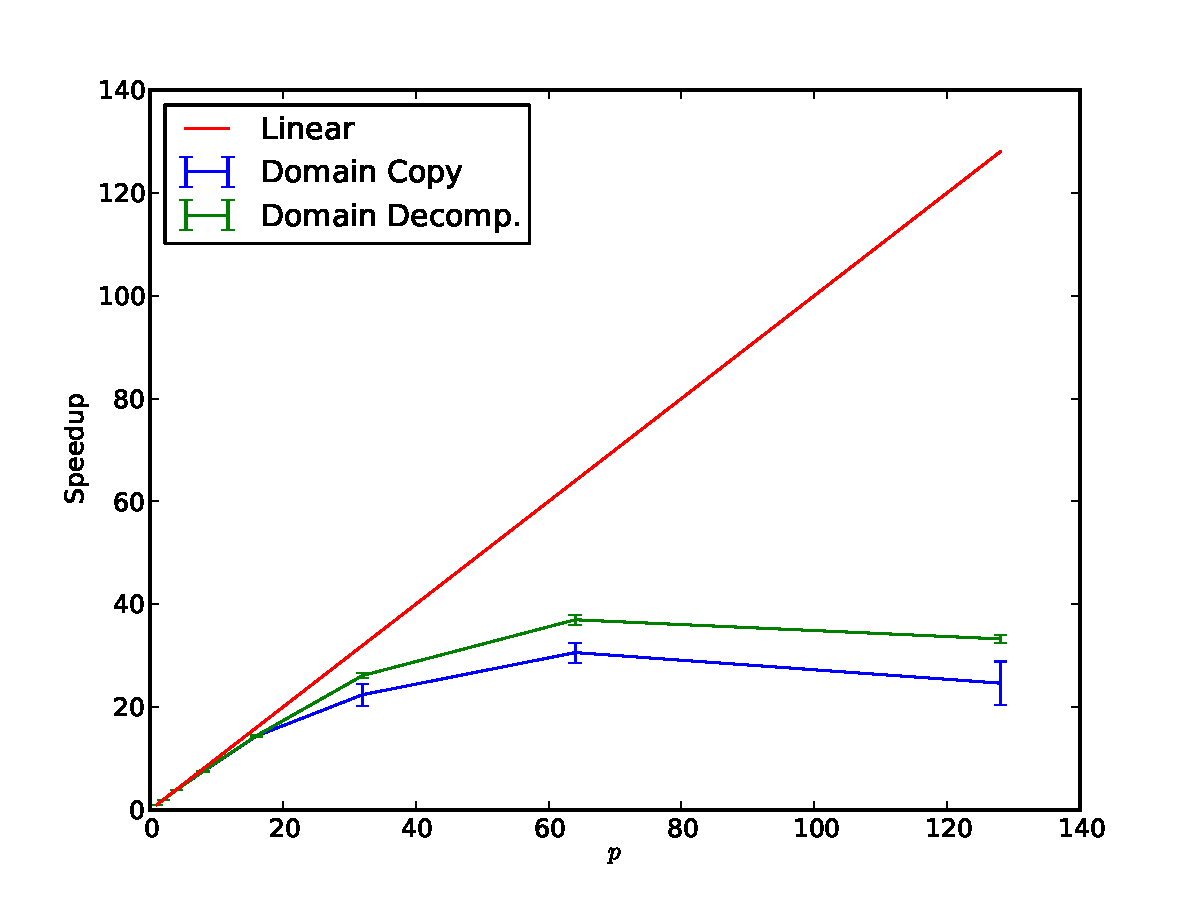
\includegraphics[width=1.08\textwidth]{speedup_thick.pdf}
           \caption{Strong scaling to 128 processors.}
     \end{subfigure}
     \begin{subfigure}{0.5\textwidth}
         \centering
           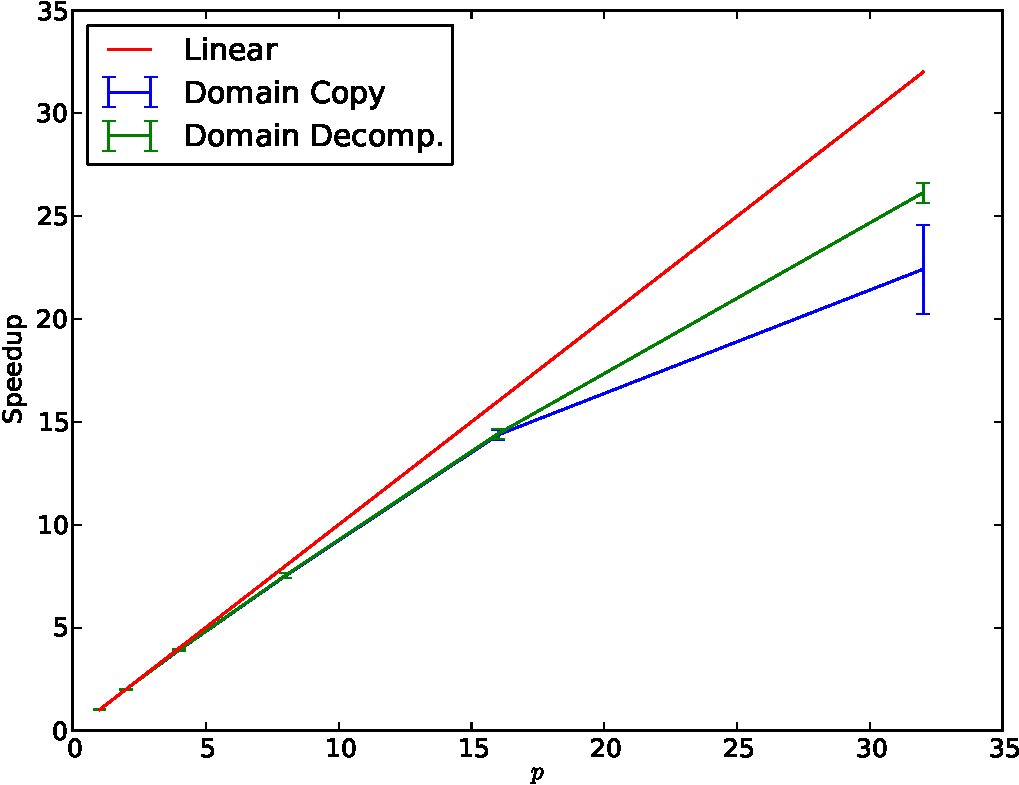
\includegraphics[width=1.08\textwidth]{speedup_zoom_thick.pdf}
           \caption{Zoomed view}
     \end{subfigure}
     \caption{For the optically \emph{thick} problem, a plot of speedup versus number of processors $p$ for $N=5\times
               10^6$ histories.\label{thicksu}}
 \end{figure}
     \begin{figure}[htbp!]
         \begin{subfigure}{0.5\textwidth}
         \centering
           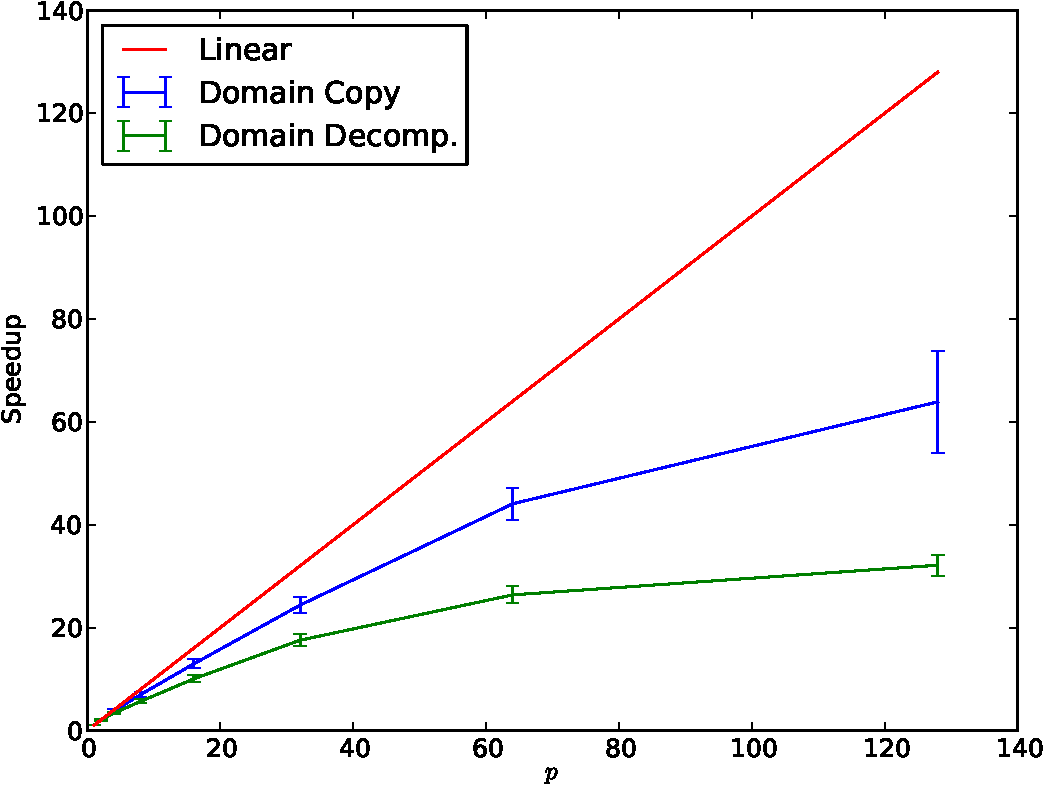
\includegraphics[width=1.08\textwidth]{speedup_thin.pdf}
           \caption{Strong scaling to 128 processors.}
     \end{subfigure}
     \begin{subfigure}{0.5\textwidth}
         \centering
           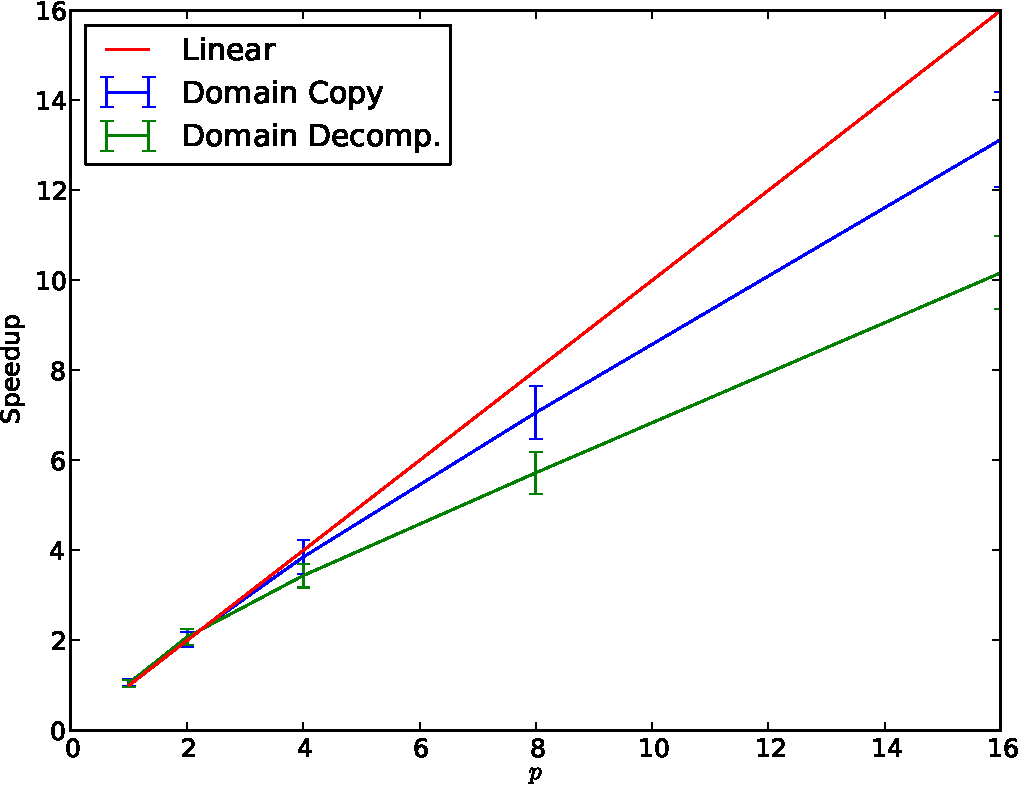
\includegraphics[width=1.08\textwidth]{speedup_zoom_thin.pdf}
           \caption{Zoomed view}
     \end{subfigure}
           \caption{For the optically thin problem, a plot of speedup versus number of processors $p$ for $N=5\times
               10^6$ histories.\label{thicksu}}
 \end{figure}

\clearpage

\subsection{Weak Scaling Study}

A plot of the weak scaling efficiency for various thread counts for the OpenMP and
MPI algorithms are given below.  In general, the weak scaling does not perform well for either
algorithm.  From 2-8 cores, the weak scaling efficiency are very similar for both the
MPI and OpenMP algorithm.  As noticed, the efficiency drops significantly from 2 to 8 cores.   The large initial
drops in the efficiency at low core counts are likely due to memory access times, as
there is minimal communication cost at these low core counts.   If the cause of the initial drop in efficiency at low core counts can be mitigated, it is likely the case that the total
efficiency would scale much better because this issue likely is effecting the
processors on all nodes locally.

For the MPI algorithm, the efficiency begins to level off at around 20\% above 16 cores.  It is noted however,
that above $\sim$32 cores, increasing the problem size, per core, does not result
in any loss in efficiency.  Although the MPI algorithm is not exceptionally
efficient, very large problems can be ran without much loss in computational time due
to additional parallel communication costs.

     \begin{figure}[htbp!]
         \centering
           %\includegraphics[width=0.75\textwidth]{openmp_weak.pdf}
           \caption{Plot of weak scaling efficiency versus $p$ for OpenMP algorithm,
               for $10^8$ integers per processor.\label{ompw}}
     \end{figure}
\begin{figure}[htbp!]
           \centering
           %\includegraphics[width=0.75\textwidth]{mpi_weak.pdf}
           \caption{Plot of weak scaling efficiency versus $p$ for MPI algorithm, for $10^8$ integers
               per processor.\label{mpiw}}
     \end{figure}
\begin{figure}[htbp!]
           \centering
           %\includegraphics[width=0.75\textwidth]{mpi_weak_small.pdf}
           \caption{Zoomed in plot of weak scaling for MPI
           algorithm, for $10^8$ integers per processor.\label{mpizoomw}}
     \end{figure}
\clearpage
\subsection{Computational time versus problem size}

Plots of computational time versus problem size, for various \emph{fixed} $p$, are
given below for each algorithm.  It is expected that the dominant term in the
time complexity for both algorithms is $O(n/p)$, so the computational times should scale linearly with $n$.
This behavior was observed, demonstrated by the linear shape of the plotted run times.
For the case of $p=4$, for MPI, there is a slight
increase at 2$\times 10^9$. This increase is the result of the problem size being at the edge of the limits
of available RAM, likely resulting in an increased time due to many off chip memory
accesses.   

As $p$ is increased, the slope of the lines decreases because the time to solve the
same size of problems with more processors should be less, as expected.
The sequential times scales as $O(n)$, and the parallel algorithms should scale with
the dominate term of $O(n/p)$, where $p$ is fixed.  Thus, the ratio of the slopes of the
serial to the parallel line should be roughly equal to $1/p$.  By visual examination, this was found to be the
case (at least generally), indicating that in fact the $O(n/p)$ term is mostly
dominant through the regime of problems tested. 

     \begin{figure}[htbp!]
         \begin{subfigure}{0.5\textwidth}
         \centering
           %\includegraphics[width=1.075\textwidth]{mpi_elems_4.pdf}
           \caption{$p=4$ \label{mpin4}}
     \end{subfigure}
     \begin{subfigure}{0.5\textwidth}
           \centering
           %\includegraphics[width=1.075\textwidth]{mpi_elems_16.pdf}
           \caption{$p=16$ \label{mpin16}}
       \end{subfigure}
        \caption{Plot of time $T_{exp}$ vs problem size $n$ for MPI
           algorithm.\label{mpin}}
     \end{figure}


\clearpage
\subsection{Determining Asymptotic Time Coefficients}

The experiment to determine the asymptotic coefficients as discussed in the
experimental set up was performed for various processor counts, for both algorithms.
Assuming the $O(n/p)$ term dominates, as demonstrated in the previous section, the plotted coefficients represent an
approximate experimental time of the form
\begin{equation}
    T_{exp}(n,p) \simeq C_{0}T_{pred}(n,p) = C_{0}\left(\frac{n}{p}\right), \quad n>n_0
    \label{duh}
\end{equation}
A table summarizing the visually estimated coefficients, for both algorithms and various $p$,  is
given in Table~\ref{tab1}. Plots of the ratio $T_{exp}/T_{pred}$ versus $n$, for
various $p$, are given below.  These plots were used to visually estimate the value
of the coefficents.  Enlarged graphs are included as necessary to 
better discern the values of data points.

As demonstrated in the table, the model in
Eq.~\eqref{duh} is fairly accurate as the coefficients generally agree, but there is
a clear trend with $p$ that is not being accounted for.  The fact that $C_0$ is increasing
with $p$ indicates that there is extra \emph{positive} terms not included in the
predicted time model $T_{pred}$.  This is not expected as $T_{pred}$ does not attempt
to include a term for the $O(p)$ or $O(\log p)$ parallel steps.   

The variablity in the threshold coefficient $n_0$ in the MPI algorithm is also a result of the lack of
including weighted $O(p)$ and $O(\log p)$ terms.  In particular, at lower values of
$n$ the ratio $T_{exp}/T_{pred}$ is above $C_0$.  This indicates that the
experimental times are much larger than $C_O(n/p)$ predicts.  Thus, at lower values of
$n$, the $O(p)$ terms are more significant (relative to the total run time) so the
$O(n/p)$ is no longer the dominant term in the time complexity.  As $p$ is increased,
the $O(n/p)$ term becomes less dominant, leading to an increased value of $n_0$. This
can be seen in particular in the $p=64$ case.  The OpenMP algorithm does not
demonstrate as much variablity in $n_0$ because $n$ is large relative to the low
values of $p$, and the shared memory allows for the simple $O(p)$ serial prefix
summation in the algorithm to be performed with relatively low performance cost.

\begin{table}[h!]
    \caption{\label{tab1} Tabulated results for estimating asymptotic coefficients}
\centering
\begin{tabular}{|c|c|c|} \hline
    $p$ & $C_0$ & $n_0$ \\ \hline
    \multicolumn{3}{|c|}{OpenMP} \\ \hline
     2 & 0.0034 & $0.1\times10^9$ \\
     4 & 0.0044 & $0.1\times10^9$ \\
     8 & 0.0075 & $0.1\times10^9$ \\ \hline
    \multicolumn{3}{|c|}{MPI} \\ \hline
     4 & 0.0044 & $0.4\times10^9$ \\
     16 & 0.0095 & $0.4\times10^9$ \\
     64 & 0.0150 & $1.0\times10^9$ \\ \hline
\end{tabular}
\end{table}
%
%     \begin{figure}[htbp!]
%         \begin{subfigure}{0.5\textwidth}
%         \centering
%           \includegraphics[width=1.075\textwidth]{openmp_asym_2.pdf}
%           \caption{$p=2$ \label{ompn2}}
%     \end{subfigure}
%         \begin{subfigure}{0.5\textwidth}
%         \centering
%           \includegraphics[width=1.075\textwidth]{openmp_asym_4.pdf}
%           \caption{$p=4$ \label{ompn4}}
%     \end{subfigure}
%     \begin{subfigure}{0.5\textwidth}
%           \centering
%           \includegraphics[width=1.075\textwidth]{openmp_asym_8.pdf}
%           \caption{$p=8$ \label{ompn8}}
%       \end{subfigure}
%     \begin{subfigure}{0.5\textwidth}
%           \centering
%           \includegraphics[width=1.075\textwidth]{openmp_asym_zoom_8.pdf}
%           \caption{$p=8$, enlarged \label{ompnzoom8}}
%       \end{subfigure}
%       \caption{Plot of $T_{exp}/T_{pred}$ vs problem size $n$ for OpenMP
%           algorithm.\label{ompn}}
%     \end{figure}
%
%
%
%     \begin{figure}[htbp!]
%         \begin{subfigure}{0.5\textwidth}
%         \centering
%           \includegraphics[width=1.075\textwidth]{mpi_asym_4.pdf}
%           \caption{$p=4$ \label{mpin4}}
%     \end{subfigure}
%     \begin{subfigure}{0.5\textwidth}
%           \centering
%           \includegraphics[width=1.075\textwidth]{mpi_asym_16.pdf}
%           \caption{$p=16$ \label{mpin16}}
%       \end{subfigure}
%     \begin{subfigure}{0.5\textwidth}
%           \centering
%           \includegraphics[width=1.075\textwidth]{mpi_asym_zoom_16.pdf}
%           \caption{$p=16$, enlarged \label{mpinzoom16}}
%       \end{subfigure}
%     \begin{subfigure}{0.5\textwidth}
%           \centering
%           \includegraphics[width=1.075\textwidth]{mpi_asym_64.pdf}
%           \caption{$p=64$ \label{mpin64}}
%       \end{subfigure}
%     \begin{subfigure}{0.5\textwidth}
%           \centering
%           \includegraphics[width=1.075\textwidth]{mpi_asym_zoom_64.pdf}
%           \caption{$p=64$, enlarged \label{mpinzoom64}}
%       \end{subfigure}
%       \caption{Plot of $T_{exp}/T_{pred}$ vs problem size $n$ for MPI
%           algorithm.\label{mpin}}
%     \end{figure}

\section{Conclusions}

The various experiments performed were able to provide insight into the performance
of the two algorithms.  Both algorithms were able to demonstrate speedup
over the serial algorithm.  Although the weak scaling studies did not show very good efficiency,
they did demonstrate that the algorithms can be used to solve large problems that a
serial algorithm could not necessarily handle.  The time complexity experiment
demonstrated that in general for parallel algorithms the dominant parallel $O(n/p)$
terms can provide a good estimate of scaling with $n$, but may not be sufficiently
accurate across a large range of $p$. Also, the weak scaling experiment demonstrated that there is extra costs that we are
clearly not accounting for in our model. In general, because the prefix sum involves such primitive operations, it exposed any memory or
other overhead in computations, even at relatively large input sizes of
$\mathcal{O}(10^9)$ integers.  This caused the need for very efficient code to demonstrate speed
up. 

Overall, the MPI algorithm is a better choice over OpenMP, at least for this
machine and sufficiently large values of $n$.  The MPI algorithm showed similar, or slightly better,
performance at low thread counts than OpenMP, for all experiments performed.  In
addition, it can easily be extended to large
core counts without the need for shared memory.  On a machine that did not have the
issue of non-uniform RAM access times across multiple chips,
the OpenMP algorithm may show better performance at low core counts. The OpenMP
algorithm may also perform better at lower values of $n$ that were not thoroughly
tested in the experiments.  The results of the asymptotic
complexity experiments indicate that the value of $n_0$ is generally larger for the
MPI algorithm.  Once $n$ is large enough, this fixed cost of the MPI
communication, per $p$, is negligible.  Although the OpenMP algorithm has a
similar overhead due to the cost of managing threads, it is not quite as large. 


BETTER TO HAVE EDGE PROCESSORS OWN MORE DOMAIN

For the thin problem, probability of going whole way is 0.41

\end{document}



